\documentclass[]{article}
\usepackage{lmodern}
\usepackage{authblk}
\usepackage{amssymb,amsmath}
\usepackage[T1]{fontenc}
\usepackage[utf8]{inputenc}
\usepackage[margin=1in]{geometry}
\usepackage{hyperref}
\hypersetup{unicode=true,pdftitle={multicorner.py: pairplots for multi-modal distributions},pdfborder={0 0 0},breaklinks=true}
\urlstyle{same}  % don't use monospace font for urls
\usepackage{graphicx}
\setlength{\parindent}{0pt}
\setlength{\parskip}{6pt plus 2pt minus 1pt}
\setlength{\emergencystretch}{3em}  % prevent overfull lines
\providecommand{\tightlist}{\setlength{\itemsep}{0pt}\setlength{\parskip}{0pt}}
\setcounter{secnumdepth}{0}

\title{multicorner.py: pairplots for multi-modal distributions}
\author{Zachary Murray}
\affil{Research Excellence Fellow, Université Côte d'Azur}
\date{\today}

\begin{document}
\maketitle

%\textbf{Paper DOI:} \url{INSERT if Accepted}\\
\textbf{Software Repository:} \url{https://github.com/dfm/corner.py}\\
%\textbf{Software Archive:} \url{INSERT if Accepted}\\

\section{Summary}\label{summary}

Pairplots (also known as Corner Plots and Scatterplot matrices) are one of the best ways of visualizing high dimensional data.
Starting with \emph{corner.py} (originally \emph{triangle}) by Dan Foreman-Mackey (Foreman-Mackey 2016), corner plots have been used extensively in all fields of the physical and computer sciences for visualizing high dimensional data, especially the output of MCMC chains and other sampling methods \cite{corner}. 

The result is the production of several simmilar packages, all specialized to create corner plots for one application or another, for example, ChainConsumer \cite{Hinton2016}, specialized in processing EMCEE or other sampling method output, whose greatest advantages include the ability to sample multimodal posteriors. Seaborn, used for machine learning, also includes a pair plot alternative as part of its packaging \cite{seaborn}. Pairplors.jl is a solution for Julia users \cite{pairplotsjl}.

Other packages, like cornerhex \cite{cornerhex}, improve on the same concept by representing the density distribution using hexagonal, rather than square bins, as hexagonal bins - being more circular - result in greater effective packing efficiency and less distortion \cite{Carr_1987}. 

However, whether applied to MCMC samples, or multivariate data generally, all these approaches are less effective when there is a significant separation in scale between individual modes of a posterior and the distances between them.  Fortunately, this type of strong scale-separation is ideal for clustering algorithms. Multicorner is a highly customizable package that mixes the visualization of capabilities of corner/pairplots with clustering algorithms to visualize highly multimodal and multidimensional datasets.


\section{Statement of Need}\label{statement-of-need}

Corner plots featuring widely separated yet compact distributions are relatively rare compared to single-modal cases but still occur frequently across various scientific fields. Such distributions often arise in periodic models when datasets lack sufficient information to constrain periodicity. For example, this issue can manifest in orbital parameter estimation \cite{Blunt_2017}, the determination of asteroid pole orientations \cite{Magnusson_1986}, but are not exclusive to them and can also occur in non-periodic scenarios such as spectroscopy \cite{Damiano_2023}.

More broadly, multimodal distributions may also result from underestimated error bars \cite{Hogg_2010}, often due to unaccounted-for or underestimated systematic errors. As astronomical observations improve in quality and characterization while random errors decrease, systematic uncertainties will play an increasingly critical role in data analysis.

Furthermore, scale separation is a common phenomenon in large datasets. For example, in geographic data, tightly clustered points (e.g., within cities) may be separated by vast distances, coral reefs may be distributed across large oceanic expanses, and similar scale-separated patterns emerge in various domains. Given the prevalence of such scale-separated distributions, a dedicated visualization tool is urgently needed.


The following is a simple demonstration of a visualization made with \emph{multicorner}:


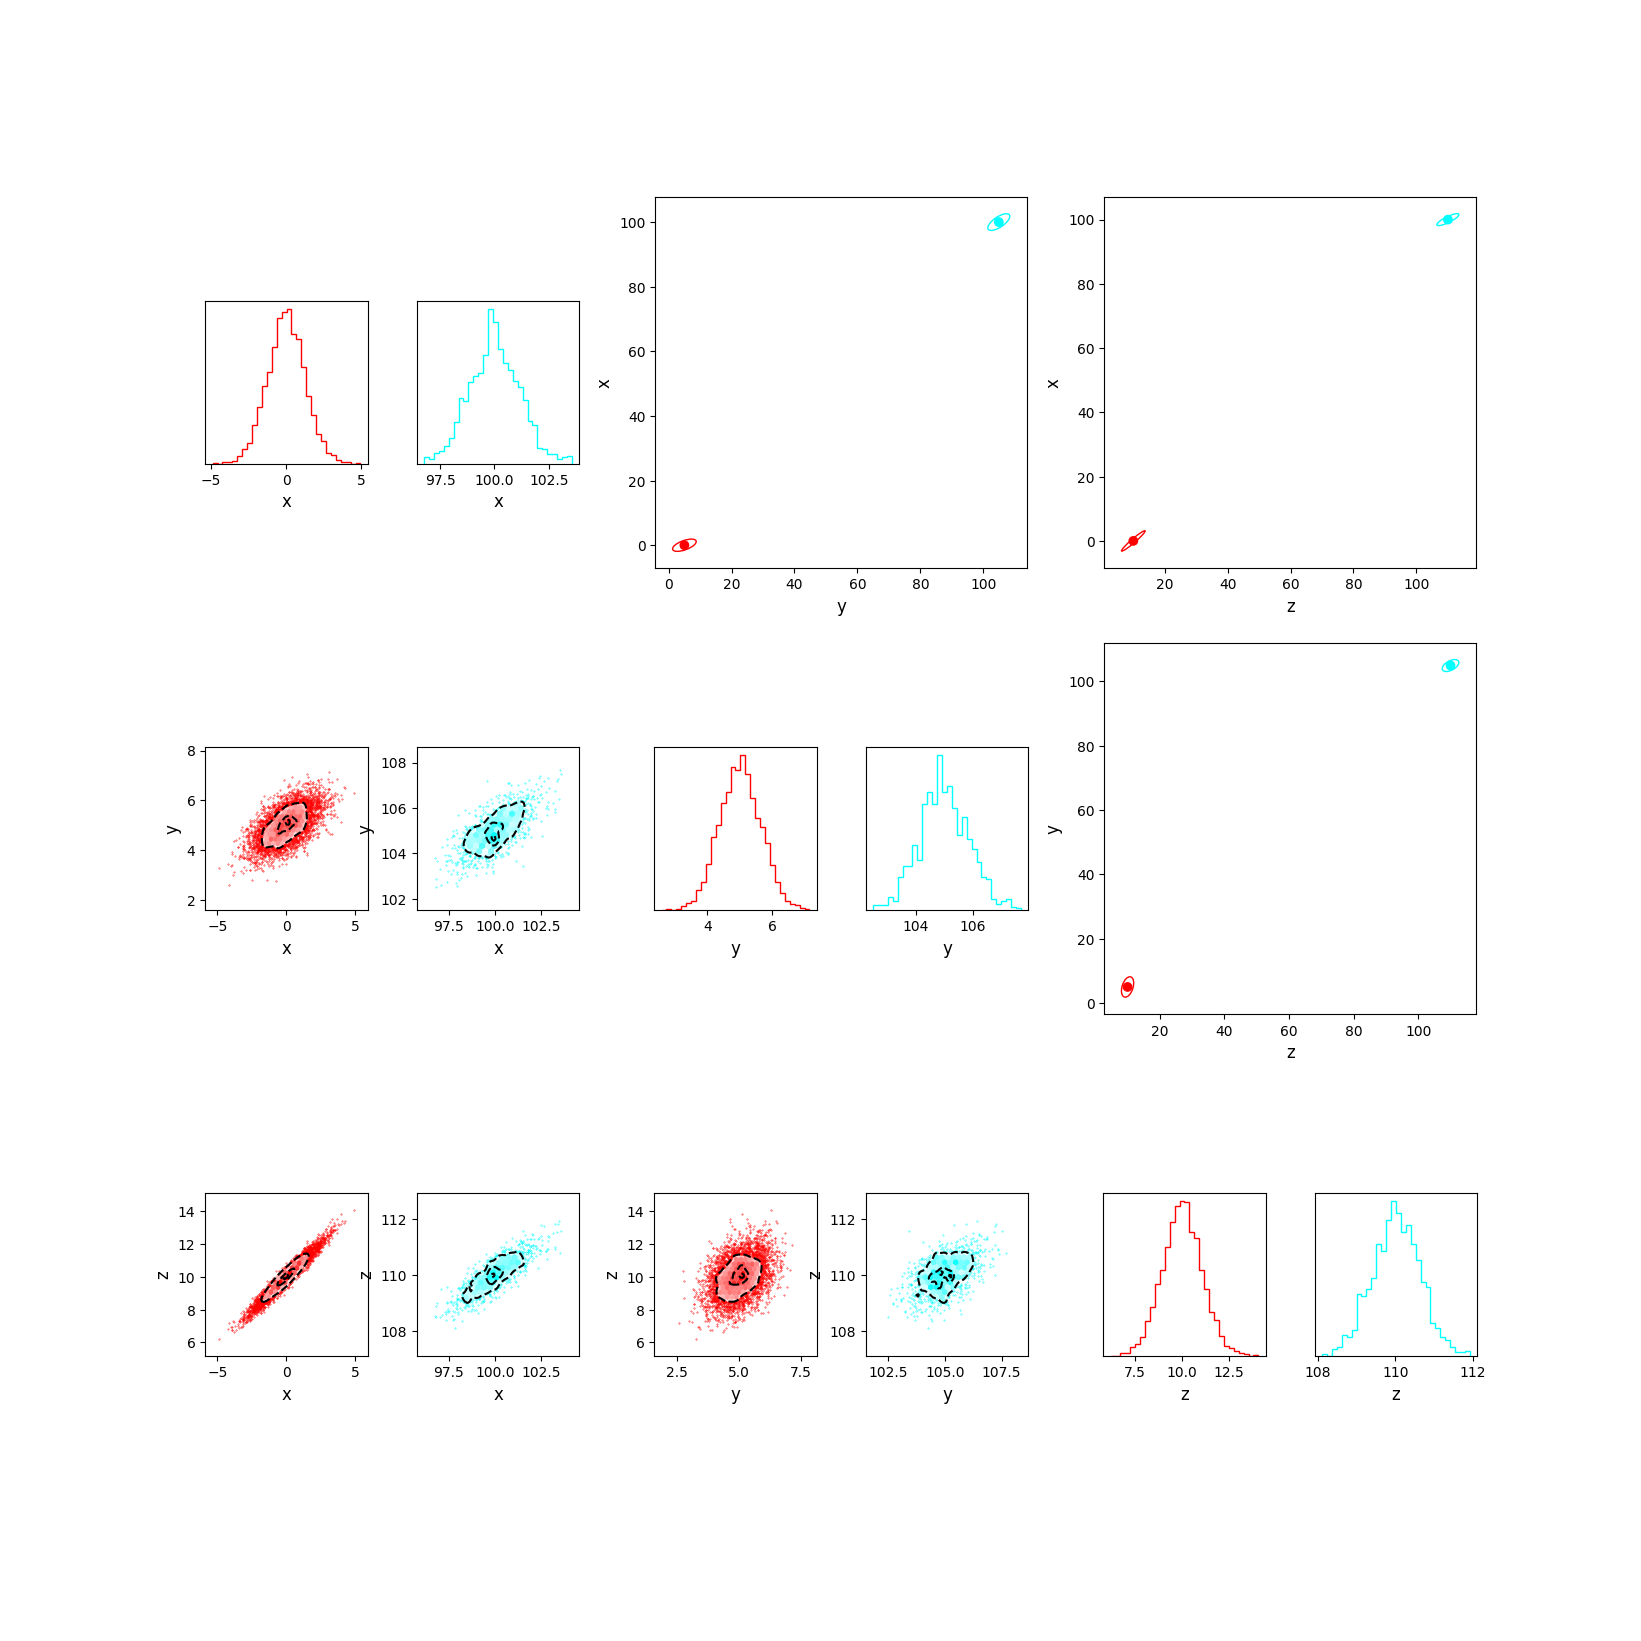
\includegraphics[width=1.0\textwidth]{multicornerplot.png}

And a visualization using \emph{corner.py} for comparison.

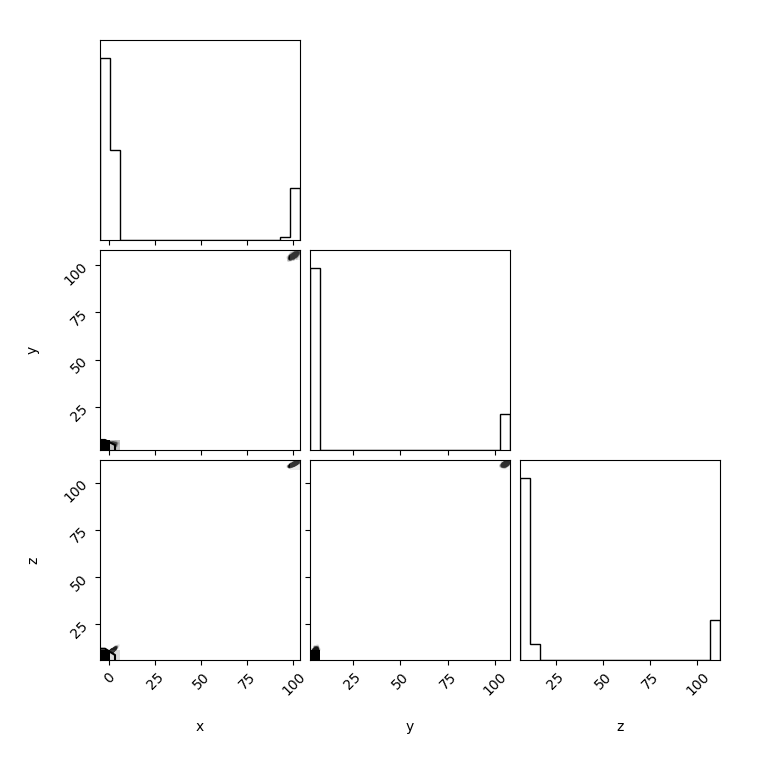
\includegraphics[width=1.0\textwidth]{cornerplot.png}


\section{Reading the Plot}\label{reading_the_plot}

These plots, produced by \emph{multicorner}, are divided into three main parts.

\begin{enumerate}
    \item \textbf{The lower triangle} – Much like a traditional corner plot, the lower triangle presents information about each distribution in a grid of subplots. These are equivalent to a corner plot for each individual \textit{mode} that makes up the dataset.

    \item \textbf{The diagonal} – The diagonal displays histograms of each individual \textit{mode} in the dataset, similar to a traditional corner plot.

    \item \textbf{The upper triangle} – The upper triangle illustrates the relative positions of the \textit{modes} within the dataset. It provides insight into the large-scale distribution of data, whereas the diagonal and lower triangle highlight smaller-scale details. Since it focuses only on large-scale features, the lower triangular panel can be scaled to give a sense of the relative orientation of the covariances between modes.
\end{enumerate}

\bibliographystyle{unsrt}  
\bibliography{references}

\end{document}
